\documentclass[10pt,letterpaper]{article}
\usepackage[top=0.85in,left=2.5in,footskip=0.75in]{geometry}
%\usepackage[top=0.85in,left=2.75in,footskip=0.75in]{geometry}
\usepackage{amsmath,amssymb}
\usepackage{changepage}
\usepackage[utf8x]{inputenc}

\usepackage{textcomp,marvosym}
\usepackage{nameref,hyperref}


\usepackage{microtype}
\DisableLigatures[f]{encoding = *, family = * }

\usepackage[table]{xcolor}

\usepackage{booktabs}

\usepackage{array}

\newcolumntype{+}{!{\vrule width 2pt}}

\newlength\savedwidth
\newcommand\thickcline[1]{%
  \noalign{\global\savedwidth\arrayrulewidth\global\arrayrulewidth 2pt}%
  \cline{#1}%
  \noalign{\vskip\arrayrulewidth}%
  \noalign{\global\arrayrulewidth\savedwidth}%
}

\newcommand\thickhline{\noalign{\global\savedwidth\arrayrulewidth\global\arrayrulewidth 2pt}%
\hline
\noalign{\global\arrayrulewidth\savedwidth}}

\raggedright
\setlength{\parindent}{0.5cm}
\textwidth 5.25in 
\textheight 8.75in

\usepackage[aboveskip=1pt,labelfont=bf,labelsep=period,justification=raggedright,singlelinecheck=off]{caption}
\renewcommand{\figurename}{Fig}

\usepackage{subcaption}

\bibliographystyle{plos2015}

\makeatletter
\renewcommand{\@biblabel}[1]{\quad#1.}
\makeatother

\usepackage{lastpage,fancyhdr,graphicx}
\usepackage{epstopdf}
%\pagestyle{myheadings}
\pagestyle{fancy}
\fancyhf{}
\rfoot{\thepage/\pageref{LastPage}}
\renewcommand{\headrulewidth}{0pt}
\renewcommand{\footrule}{\hrule height 2pt \vspace{2mm}}
\fancyheadoffset[L]{2.25in}
\fancyfootoffset[L]{2.25in}
\lfoot{\today}

\usepackage{cite}
\usepackage{ragged2e}
\usepackage{multirow}

\begin{document}
\vspace*{0.2in}

\justify

% Title must be 250 characters or less.
\begin{flushleft}
{\Large
\textbf\newline{Estimation of Echinococcosis Cyst Prevalence in Two Rural Communities Considering spatial distribution in the selection bias} % Please use "sentence case" for title and headings (capitalize only the first word in a title (or heading), the first word in a subtitle (or subheading), and any proper nouns).
}
\newline
% Insert author names, affiliations and corresponding author email (do not include titles, positions, or degrees).
\\
O G E Espinoza-Hurtado\textsuperscript{1*},
E A Chacón-Montalvan\textsuperscript{2},
Saúl Santivañez\textsuperscript{1,3}
%Name4 Surname\textsuperscript{2},
%Name5 Surname\textsuperscript{2\ddag},
%Name6 Surname\textsuperscript{2\ddag},
%Name7 Surname\textsuperscript{1,2,3*},
%with the Lorem Ipsum Consortium\textsuperscript{\textpilcrow}
\\
\bigskip
\textbf{1.} Global Health Center, Cayetano Heredia Peruvian University, Lima, Peru
\\
\textbf{2.} Mathematics and Statistics Department, Lancaster University, Lancaster, United Kingdom
\\
%\textbf{3} Research Center on Modeling Random Phenomena and Complex Systems, National University of Engineering, Lima,  Peru
%\\
\textbf{3.} National University of the Center of Peru, Junin,  Peru
\\

\bigskip

* oespinozah@uni.pe

\end{flushleft}

\section*{Abstract}
\textbf{Objective:} Determine a correction factor to correctly estimate the prevalence of hydatidosis. \textbf{Methods.} Prevalence was estimated by weighted likelihood. Each point was considered as a realization of a Poisson process (marked for the case of the sample). Intensity functions were estimated as Poisson process. Risk function was estimated using a GAM Weighted of binomial family and logistic transformation as link function. La correct value of $\rho$ was the OR of the disease between the sample and the population. \textbf{Results and Discussion.} The correction factor was 1.216 and with it there was a fixed prevalence of 0.207. The intensity graphs show that the overestimation could have been due to an overcollection of cases at certain points. Georeferencing could become an alternative to avoid overestimating without expanding coverage sampling. \textit{\textbf{Keyword:} Hydatidosis prevalence, Spatial distribution, Sample selection bias correction, Re-weighting}.

\section*{Introduction}
% Principal objective:
% - Estimate prevalence under sampling bias in a rural city in Junin
% Specific objects:
% - Determine the correction of case-control studies under bias samplingtia
% - Propose a spatial marked point process model
% - Estimate prevalence using the bias-corrected spal model

% Importance of epidemiological indicators and common challenges
Correctly estimate epidemiological indicators of a disease is of utmost importance for a country. This because of the impact generated by a zoonosis on the economy of a society consists not only of the money invested for its treatment and prevention or the losses that it causes in livestock and agricultural activities; but also includes disability and lifestyle change that it and his treatment entails~\cite{shaw2017dalys}. Some diseases, for example hydatidosis~\cite{santivanez2010factores}, are endemic in certain regions. Therefore, they are considered as a public health problem and the underestimation or overestimation of their effects and scope have an impact on their control~\cite{moro2011economic}.


% Prevalence and spatial prevalence: possible biases and common approaches
In prospective cohort studies conducted in a community there is often a selection bias (bias given by a systematic error in the collection~\cite{celentano2019gordis}). When sampling is done for convenience, the ratio of cases and controls could be different between the sample and the population. As a result, the traditional way to estimating  prevalence as a proportion~\cite{scheaffer2006elementary}, where $n_1$ and $n_2$ are the number of cases and controls in the sample, would determine an incorrect value for it.
\begin{equation}
    \hat{\theta} = \frac{n_1}{n_1 +  n_2}
\end{equation}
% Problem description: campaigns, biases, common approaches are wrong
The over-collection of cases in the sample may be due to their predisposition to participate in the study. But it can also be given by the location of the health center where the information was collected.
% Explain the context of your city and the associated disease (motivating case of study)
% Example of a common bias? I am not sure
In the case when the bias effect is significant, it is necessary to integrate a correction factor $\rho$ in the estimation based on the Weighted Likelihood Estimation for a Bernoulli distribution.
\begin{equation}\label{WLE}
    \tilde{\theta} = \frac{n_1}{n_1 + \rho \; n_2}
\end{equation}

% Common current approaches to fix the possible biases (competing with your approach), disadvantages, what is wrong
% capture-recapture, propensity score, Bayesian models, etc.
% what is missing?
% Other approaches
Several studies have tried to fix the bias under other approaches and for other purposes. A study on hydatidosis have used the propensity score as a tool to fix bias in order to estimate OR; but not the prevalence~\cite{malki2014}. In contrast, a study carried out in China~\cite{bailly2015bayesian} considered the heterogeneity of the probability that each individual has to be selected for a sample in estimating the number of cancer patients, treating the information obtained under a Bayesian approach for a case of recapture and recapture. The limitation of this study is the need to have a very large area and more than one health center in it. By other hand, considering the spatial distribution of the individuals captured in a given sample has been used in the field of ecology~\cite{Royle2014Spatial}, which can be replicated in the field of epidemiological sciences~\cite{braeye2016capture}.

% Present clearly your goal!
% Your approach: spatial marked point processes with additive (non-linear) effects: advantages and other aspects to call the attention of readers
% With the goal of estimating hidatidosis prevalence in XXXX under bias sampling, we propose a spatial marked point processes with additive effects that is able to take into acount the trends ....
With the goal of estimating hidatidosis prevalence in Corpacancha we propose a spatial marked point processes with additive effects that is able to take into acount the trends. For that, was necessary determine the correction of case-control studies under bias sampling proposing a spatial marked point process model. In addition, this method could be used in other studies with similar characteristics in its collection.

% Paper's structure
In materials and methods section, the population was presented and the information gathering process was detailed, and the statistical analysis used is described. Also, the usefulness of the method for other studies is mentioned.
In results and discussion section the analysis results are displayed together with graphs in order to compared with traditional methods

%\newpage
\section*{Materials and methods}

\subsection*{Population under study}
The population under the study is composed of the 332 (141 at sample) citizens of Corpacancha, Junin - Peru. For this case, the study did not consider within the population those who live in the slaughterhouse because they are very far from the health center.

%\begin{figure}[h]
%\centering
%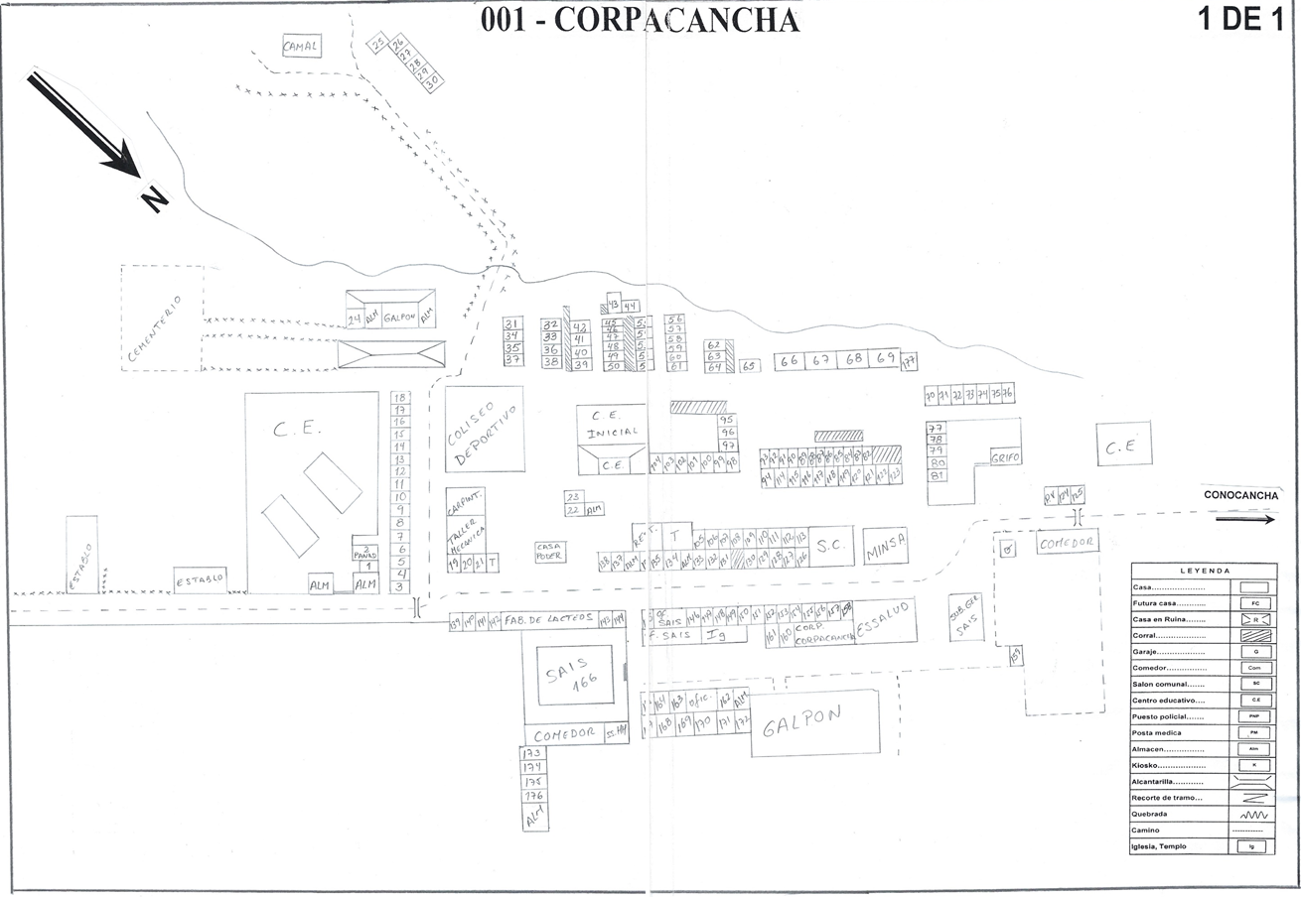
\includegraphics[width=0.75\textwidth]{images/corpacancha_mapa.png} %,angle=180
%\caption{Urban map of Corpacancha (Junin, Peru)}
%\end{figure}
%Characteristics

\subsection*{Design and sampling}
It was a prospective cohort study that began in October 2017.
It had 2 different ways, one after the other, to obtain the baseline information from the citizens. The first one consisted of a free health campaign to diagnose and rule out hydatidosis in the village health center. In which to determine the presence of hydatidosis in each patient, an abdominal ultrasound (according to WHO criteria~\cite{who2003international}) and a western blot serological test were performed~\cite{davelois2016rendimiento}. The second consisted in searching for positive cases directly in the community. In that, georeferencing of each household was made by a census conducted a few months after the health campaign. In this study, the outcome only measured the presence of hydatidosis and did not make a difference between the affected organ (liver or lung). Some missing data respect aged (less than 4 observation) have been inputted using mean.

%collecting the information through

\subsection*{Statistical analyses}
First, the statistical analysis began describing the campaign information and covariates to deteterminate which on has an effect in the prevalence and how work with their values.

Then, taking into consideration that each point ($x_i = \left\{x_{i1}; x_{i2} \right\} \in R^2$) have been considered as a realization of a Poisson process~\cite{baddeley2015spatial}, it began with an exploratory spatial analysis of the data (intensity with contours) to show the proportion between the sample intensity $\lambda$ and the population intensity $\lambda_p$. Then, it adjusts the intensity function of the sample by
\begin{align*}
	\lambda(x_i) &= \lambda_p(x_i) h(x_i)\\
	&= \lambda_p(x_i) exp \left(\beta_0 + h'(x_i)\right)\\
	\log \lambda(x_i) &= \log \lambda_p(x_i) + \beta_0 + h'(x_i)
\end{align*}
Using a generalized additive model (GAM), where $\log \lambda_p(x_i)$ is an offset, $\beta_0$ is a constant and $h(x_i)$ is the sampling effort por each $x_i$ point. If $h'(x_i) = 0$, $\log \beta_0$ is the sampling proportion. Subsequently, the sample risk function $\pi(x_i)$ was estimated using a GAM Weighted of binomial family and logistic transformation as link function~\cite{friedman2001elements} with $\lambda_p(x_i)/\lambda(x_i)$ as weight for each $x_i$. For this model, it considered both the special effect and other covariates that may explain the presence of the disease optimizing the model's auc. With this rick function, disease was predicted for each unsampled individual. This prediction of unsampled cases and controls is because the optimal value of $\rho$ is given when it is equal to the OR of the disease between the sample and the population.
\begin{equation*}
    \rho = OR_{sample,population}
\end{equation*}
Finally, the value of $\rho$ was used in Eq \ref{WLE} to estimate unbiased prevalence.
\subsection*{Method application}
%Add in which cases the method can be used
The importance of using this method lies in the time space between the two data collection. The corrected value of the prevalence using the data from the campaign and the census, together with the other processed information, can be used as a reference indicator when the principal investigator need to determinate the budget about the second stage of collection.

%\newpage


% Results and Discussion can be combined.
\section*{Results and Discussion}
The health campaign obtained a coverage of 42.5\%, showing a prevalence of hydatidosis of 0.241 (IC$_{95\%} \left[ 0.189; 0.293 \right] $). As Table \ref{covariates} shows, there is a bit observable difference from disease in covariates.
\begin{table}[htbp]
  \centering
    \begin{tabular}{llll}
    \toprule
    \textbf{Covariate} &       & \multicolumn{1}{c}{\textbf{Positive}} & \multicolumn{1}{c}{\textbf{Negative}} \\
    \midrule
    \multicolumn{2}{l}{Sex} &       &  \\
          & \multicolumn{1}{c}{Male} & \multicolumn{1}{c}{16 (27.6\%)} & \multicolumn{1}{c}{42 (72.4\%)} \\
          & \multicolumn{1}{c}{Female} & \multicolumn{1}{c}{18 (21.7\%)} & \multicolumn{1}{c}{65 (78.3\%)} \\
    \midrule
    \multicolumn{2}{l}{Age*} & \multicolumn{1}{c}{36.1} & \multicolumn{1}{c}{32.4} \\
    \midrule
    \multicolumn{2}{l}{Number of dogs} &       &  \\
          & \multicolumn{1}{c}{0} & \multicolumn{1}{c}{21 (22.1\%)} & \multicolumn{1}{c}{74 (77.9\%)} \\
          & \multicolumn{1}{c}{1} & \multicolumn{1}{c}{2 (13.3\%)} & \multicolumn{1}{c}{13 (86.7\%)} \\
          & \multicolumn{1}{c}{2} & \multicolumn{1}{c}{3 (17.6\%)} & \multicolumn{1}{c}{14 (82.4\%)} \\
          & \multicolumn{1}{c}{3} & \multicolumn{1}{c}{7 (63.6\%)} & \multicolumn{1}{c}{4 (36.4\%)} \\
          & \multicolumn{1}{c}{4} & \multicolumn{1}{c}{1 (33.3\%)} & \multicolumn{1}{c}{2 (66.7\%)} \\
    \midrule
    \multicolumn{4}{l}{* mean by result} \\
    \end{tabular}%
  \caption{Covariates}
  \label{covariates}%
\end{table}%

The coverage could be spatially presented as the proportion between the sample intensity function and the population intensity function. As show Fig \ref{samp_eff}, coverage is not constant in the space.
\begin{figure}[h]
\centering
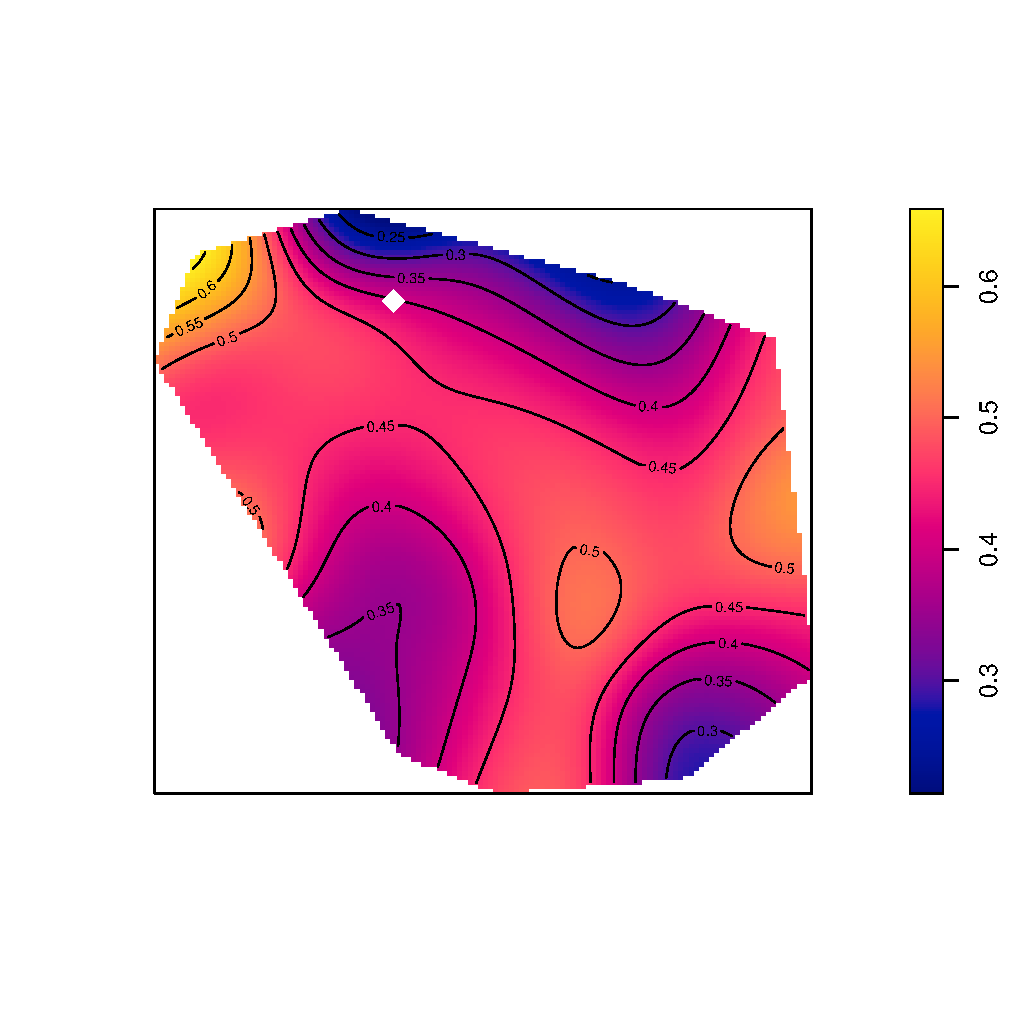
\includegraphics[width=9cm]{images/sampling_effort.pdf}
\caption{{\bf Sampling effort.} Proportion between the sample intensity function and the population intensity function where the white point is the town's health center.}
\label{samp_eff}
\end{figure}

The sampling intensity and the sampling effort (Eq. \ref{lambda}) were determinate by a GAM with 49 base functions. It made possible to fit a GAM about risk  considering covariate showed at Table \ref{covariates}. The model was chosen taking as criteria the AUC and Deviance Explained. With 23 base functions for the spatial effect considering sex, 11 base functions for the age considering sex and 5 base functions for the number of dog that each person have, the model had an AUC greater than 0.99. It is important to note that if this model to predict the cases and controls had not considered the spatial effect, nor the reweighting, the AUC of the model would have been 0.80. 
\begin{table}[]
	\centering
	\label{model_metricas}
	\begin{tabular}{@{}lcccccc@{}}
		\toprule
		\multicolumn{1}{c}{\multirow{2}{*}{Model}} & \multicolumn{3}{c}{Train}                          & \multicolumn{3}{c}{Test}            \\ \cmidrule(l){2-7} 
		\multicolumn{1}{c}{}                        & Spef. & Sens. & \multicolumn{1}{c|}{AUC}    & Spef. & Sens. & AUC    \\ \midrule
		\multicolumn{1}{l|}{Age}            & 1             & 0.0833       & \multicolumn{1}{c|}{0.5578} & 0.03125       & 1            & 0.5672 \\
		\multicolumn{1}{l|}{Age*}        & 0.9333        & 0.2917       & \multicolumn{1}{c|}{0.6122} & 0.59375       & 0.6          & 0.6453 \\
		\multicolumn{1}{l|}{Sex}            & 1             & 0            & \multicolumn{1}{c|}{0.5358} & 1             & 0            & 0.5469 \\
		\multicolumn{1}{l|}{Sex*}        & 1             & 0            & \multicolumn{1}{c|}{0.4642} & 1             & 0            & 0.5469 \\
		\multicolumn{1}{l|}{Dogs}          & 0.9333        & 0.3333       & \multicolumn{1}{c|}{0.6333} & 0.9688        & 0            & 0.149  \\
		\multicolumn{1}{l|}{Dogs*}      & 0.9333        & 0.3333       & \multicolumn{1}{c|}{0.6333} & 0.9688        & 0            & 0.149  \\
		\multicolumn{1}{l|}{Age, sex}       & 1             & 0.0833       & \multicolumn{1}{c|}{0.6369} & 0.03125       & 1            & 0.5406 \\
		\multicolumn{1}{l|}{Age, sex*}   & 0.9467        & 0.4583       & \multicolumn{1}{c|}{0.8708} & 0.5625        & 0.8          & 0.7562 \\
		\multicolumn{1}{l|}{Age, sex, dogs}        & 0.96          & 0.375        & \multicolumn{1}{c|}{0.74}   & 0.0938        & 0.9          & 0.5141 \\
		\multicolumn{1}{l|}{Age, sex, dogs*}    & 0.9467        & 0.4583       & \multicolumn{1}{c|}{0.7144} & 0.625         & 0.5          & 0.5328 \\
		\multicolumn{1}{l|}{Full}        & 0.96          & 0.333        & \multicolumn{1}{c|}{0.7403} & 0.53125       & 0.5          & 0.6    \\
		\multicolumn{1}{l|}{Full*}    & 0.9733        & 0.375        & \multicolumn{1}{c|}{0.7503} & 0.5625        & 0.8          & 0.7438 \\ \bottomrule
	\end{tabular}
	\caption{Model Fit Metrics. *Model fitted with weights.}
\end{table}
With this model, the disease was predicted to have a population size of estimated cases and controls with which the correction factor can be determined. As a result, the value of $\rho$ would be 1.346. Using this value in Eq. \ref{WLE}, the fixed prevalence was 0.191. The effect of this correction factor can be seen graphically in the change between Fig. \ref{risk_bais} and \ref{risk_unbais}.
\begin{figure}[h]
\centering
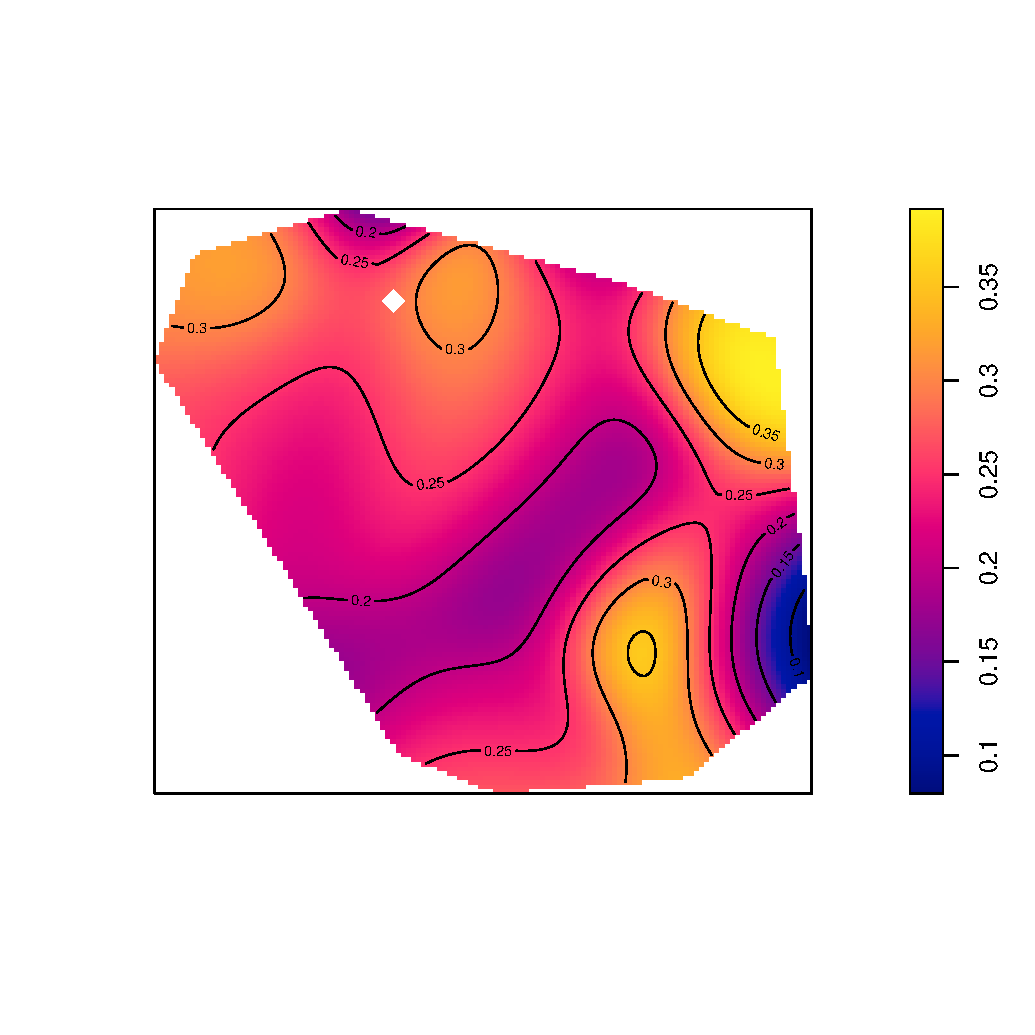
\includegraphics[width=9cm]{images/risk_bais.pdf}
\caption{{\bf Biased risk.} Risk before spatial correction.}
\label{risk_bais}
\end{figure}
\begin{figure}[h]
\centering
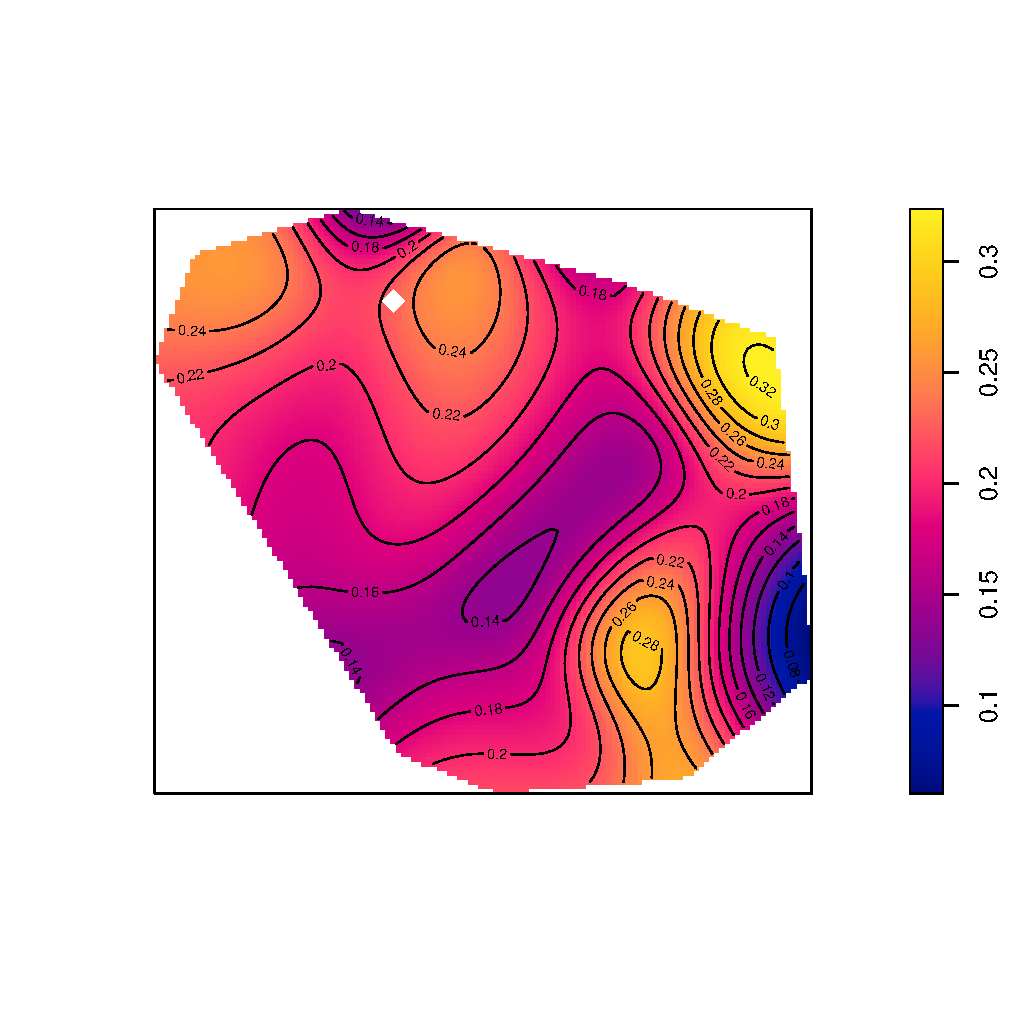
\includegraphics[width=9cm]{images/risk_unbais.pdf}
\caption{{\bf Unbiased risk.} Risk after spatial correction.}
\label{risk_unbais}
\end{figure}


A few months after the health campaign, a second data collection was carried out in the town in order to find a greater number of positive cases. In this, it was possible to increase the sampling coverage by 18 percentage points (from 42.5\% to 60.5\%). As result, hydatidosis prevalence decrease by 0.7 percentage points (from 0.241 to 0.234). It is important to show that the fixed prevalence is not closer to the prevalence after increasing coverage, than to the initial prevalence.
The result of the study shows a overestimation in the prevalence, even though increasing the sample size.

%This is because the case-control ratio of the intensities is not constant, as show Fig \ref{casecontrol}. In other words, in certain areas the intensity of cases is higher than it should. Therefore, the correction factor must necessarily be greater than 1 to correct the imbalance in the controls. 
%\begin{figure}[h]
%\centering
%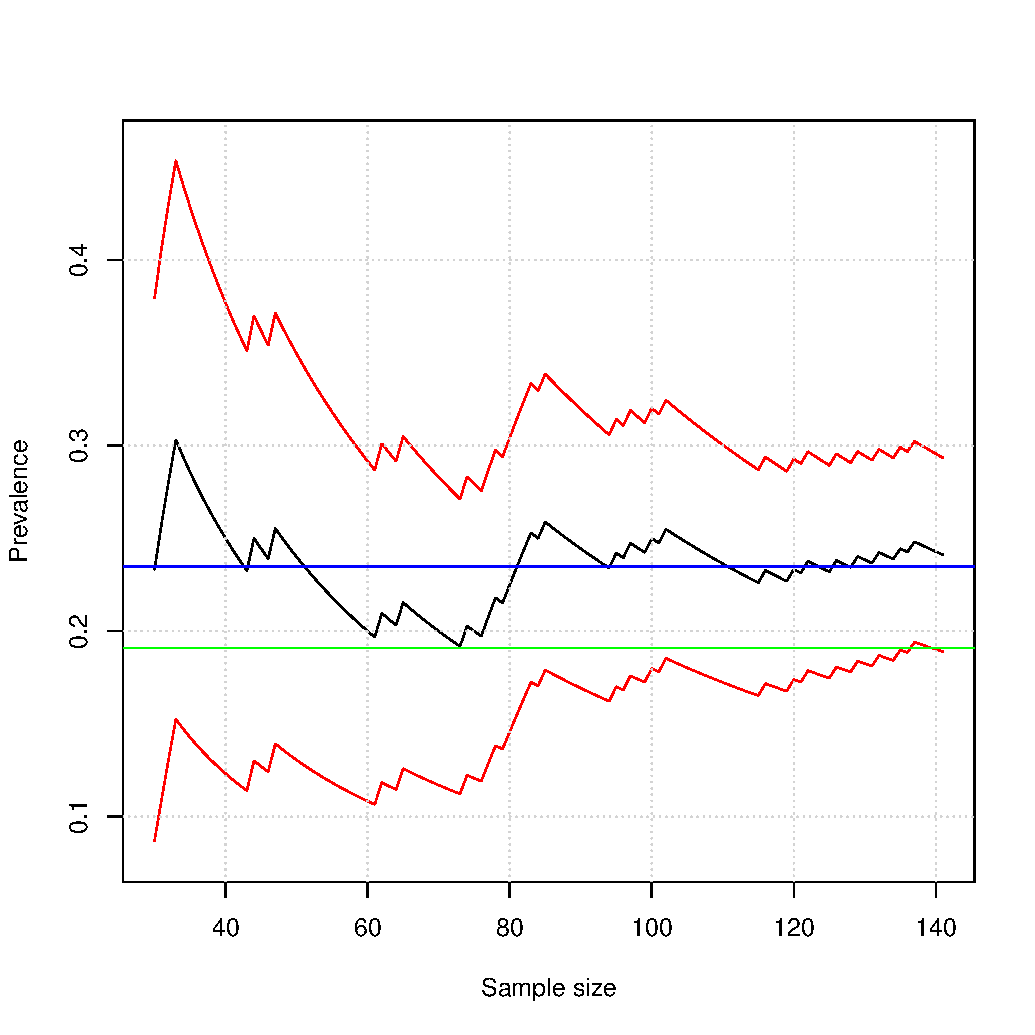
\includegraphics[width=9cm]{images/prevalence_samplesize.pdf}
%\caption{{\bf Prevalence evolution by sample size.} Black, prevalence evolution by sample size. Red, coverage interval evolution by sample size. Blue, prevalence at the second study. Green, prevalence with spatial correction}
%\label{samplesize}
%\end{figure}

\begin{figure}[h]
\centering
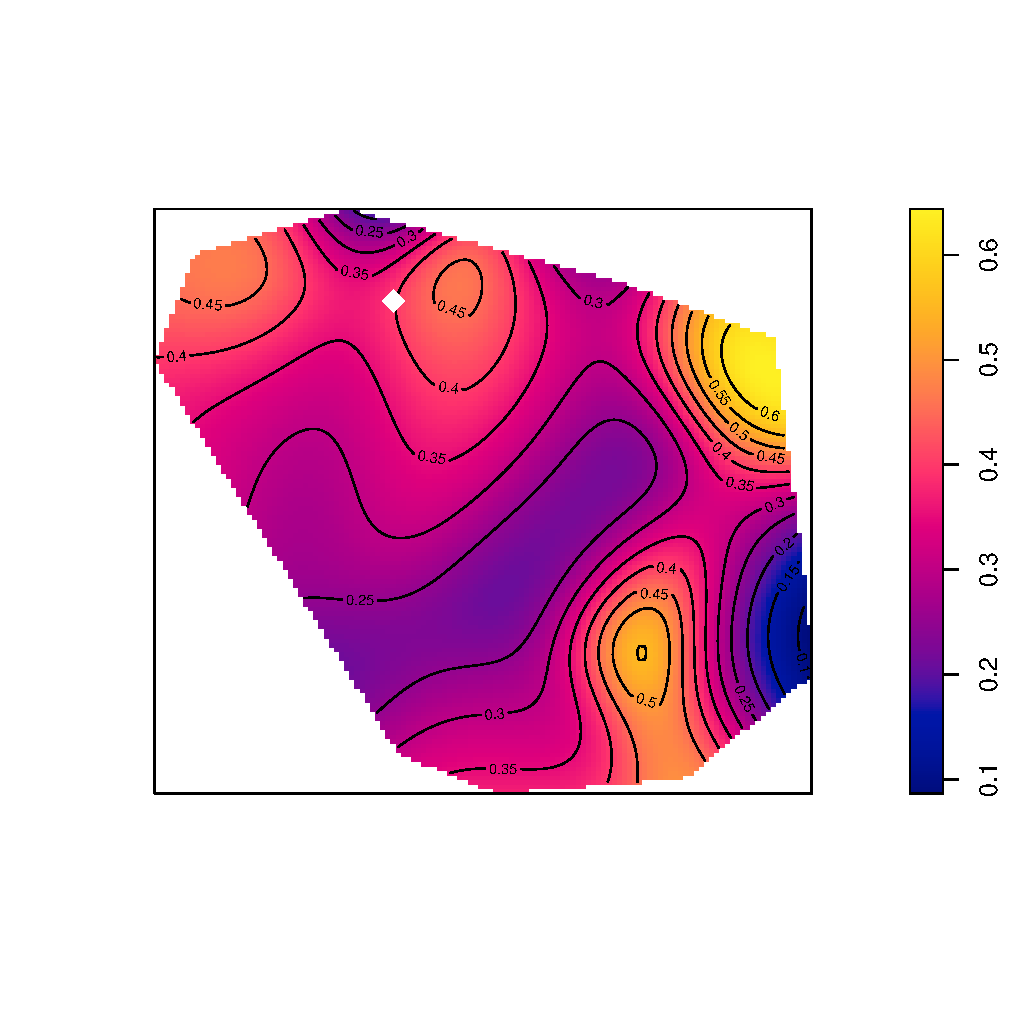
\includegraphics[width=9cm]{images/case-control.pdf}
\caption{{\bf Empirical odds function.} Proportion between cases intensity function and controls intensity function where the white point is the town's health center.}
\label{casecontrol}
\end{figure}


%\section*{Conclusion}




%\section*{Supporting information}

\section*{Acknowledgments}
The authors would like to thank the support of FONDECYT and Cayetano Heredia Peruvian University to make this paper possible


\newpage

\bibliography{references.bib}


\end{document}

